\documentclass[11pt,a4paper]{article} 

% Define page geometry
\usepackage{geometry}
\geometry{left=2.2cm,
	right=2.2cm,
	top=2.2cm,
	bottom=2cm} % Page margins
\parskip 0.15cm % Paragraph spacing
\setlength{\parindent}{0cm} % No paragraph indenting

% Text formatting
\usepackage[T1]{fontenc} % Set font
\usepackage{lineno} % Line numbers
\linespread{1.5} % Linespacing

\usepackage{amssymb}
\usepackage{multirow}
\setlength{\tabcolsep}{4pt} % Default table column sep width 

\usepackage{fmtcount}

% Image handling
\usepackage{graphicx} 
\graphicspath{ {img/} } % Define image path
\usepackage{float} % Precise figure location

% Bibliography management
\usepackage[natbib, 
	style=authoryear, 
	uniquename=false, 
	uniquelist=false,
	giveninits=true,
	dashed=false,
	maxcitenames=2, 
	mincitenames=1, 
	minbibnames=10, 
	maxbibnames=10, 
	backend=biber]{biblatex}
\renewcommand*\finalnamedelim{\addspace\&\space}
\addbibresource{phenology.bib}

% Links within document, nice figure formatting
\usepackage{xcolor}
\newcommand{\todo}[1]{\textcolor{red}{\textbf{#1}}}   % \todo{NOTE IN RED}
\usepackage[breaklinks]{hyperref}
\definecolor{links}{RGB}{0,0,0}
\hypersetup{
	breaklinks,
	colorlinks=true,
	linkcolor=links,
	anchorcolor=links,
	citecolor=links,
	filecolor=links,
	menucolor=links,
	runcolor=links,
	urlcolor=links,
	pdfauthor={John L. Godlee}
}
\def\subsectionautorefname{section}
\def\subsubsectionautorefname{section}

\newcommand{\beginsupplement}{%
	\setcounter{table}{0}
	\renewcommand{\thetable}{S\arabic{table}}%
	\setcounter{figure}{0}
	\renewcommand{\thefigure}{S\arabic{figure}}%
	}

\usepackage{makecell}

% \DeclareUnicodeCharacter{0301}{*************************************}
   
% Variables
\input{out/vars.tex}

\begin{document}

{\Large{Title: Tree species composition and diversity mediates land surface phenology in seasonally dry tropical woodlands}}

Authors: Godlee J. L.\textsuperscript{1}, Ryan C. M.\textsuperscript{1}, Siampale A.\textsuperscript{2}, Dexter K. G.\textsuperscript{1,3}

\textsuperscript{1}School of GeoSciences, University of Edinburgh, Edinburgh, EH9 3FF, United Kingdom \\
\textsuperscript{2}Forestry Department Headquarters - Ministry of Lands and Natural Resources, Cairo Road, Lusaka, Zambia \\
\textsuperscript{3}Royal Botanic Garden Edinburgh, Edinburgh, EH3 5LR, United Kingdom \\

\vspace{1em}
Corresponding author:

John L. Godlee

johngodlee@gmail.com

School of GeoSciences, University of Edinburgh, Edinburgh, United Kingdom

\section*{Acknowledgements}

\section*{Author contribution statement}

JLG conceived the study, conducted the analysis, and wrote the first draft of the manuscript. AS coordinated plot data collection in Zambia. All authors contributed to manuscript revisions. 

\section*{Data accessibility statement}

The data used in this study are from the Zambian Integrated Land Use Assessment (ILUA-II). Data were cleaned and archived by the SEOSAW project (Socio-Ecological Observatory for Studying African Woodlands). An anonymised version of the plot data are available at the following DOI: \todo{URL for Edinburgh Datashare}. Code developed for data analysis can be found here: \url{https://github.com/johngodlee/zambia_phenology}.

\newpage{}
\linenumbers

\section*{Abstract}

\begin{enumerate}
	\item{Patterns of plant phenology are a key determinant of ecosystem function. Variation in remotely sensed land surface phenology can be predicted to some extent from climate, but understanding of how ecosystem structure and plant community composition mediates patterns of land surface phenology is lacking. This impacts our ability to predict how changes in vegetation composition may affect patterns of land surface phenology, with consequences for predictions of global land-atmosphere exchange.}
	\item{We combined a dense network of \nSites{} vegetation monitoring sites across deciduous woodlands in Zambia with remotely sensed land surface phenology metrics to investigate the role of tree species diversity, composition, and woodland structure on patterns of land surface phenology, including the phenomenon of pre-rain green-up.} 
	\item{Tree species diversity was associated with earlier pre-rain green-up, a longer growing season, and a longer plateau of maximum foliage production, across all woodland types identified in the study. Increased growing season length is associated with dominance of trees from the Fabaceae, subfamily Detarioideae, which drive a longer period of maximum foliage production towards the end of the growing season. Woodland compositional types differed in their phenological patterns and biotic drivers of phenology. }
	\item{This study underlines the importance of vegetation composition and diversity as a determinant of ecosystem function, and offers new insights into the factors determining patterns of land surface phenology across the dry tropics, which are essential for realistic modelling of land-atmosphere mass and energy exchange.}
	\item{\textbf{Synthesis:} Tree species composition and diversity influence patterns of foliage production in seasonally dry tropical woodlands, with more diverse woodlands able to green-up earlier with respect to seasonal rains. Species of the Fabaceae family, subfamily Detarioideae, are associated with longer growing seasons, effectively extending the period of maximum foliage production toward the end of the growing season. Understanding variation in land surface phenology with respect to vegetation composition is of great importance for earth-system modellers aiming to parameterise predictive models of land-atmophere mass and energy exchange.}
\end{enumerate}

\newpage{}

\section{Introduction}

Plant foliage forms the primary interface between the vegetated land surface, the atmosphere and incoming solar radiation \citep{Gu2003, Penuelas2009}. Seasonal cycles of foliage production (plant phenology) play an important role in regulating global carbon, water and nitrogen cycles \citep{Richardson2013}. Terrestrial biosphere models routinely incorporate measures of plant phenology to constrain estimates of Gross Primary Productivity (GPP) (e.g. \citealt{Bloom2016}), most commonly in the form of land surface phenology products derived from remotely sensed vegetation indices as a proxy for foliage production \citep{Helman2018}. Previous studies have described environmental drivers of land surface phenology \citep{Adole2019, Guan2014}, but understanding of how the composition and structure of the vegetation itself affects patterns of land surface phenology is lacking \citep{Whitley2017}. 

At continental scales, land surface phenology can be predicted using only climatic factors, namely precipitation, diurnal temperature oscillation, and photoperiod \citep{Adole2018a, Adole2019, Guan2014}, but significant local variation exists within biomes in the timing of foliage production which cannot be attributed solely to abiotic environment \citep{Stockli2011}. It has been repeatedly suggested that the diversity, composition, and structure of plant communities plays a role in determining ecosystem response to abiotic cues driving patterns of land surface phenology \citep{Adole2018b, Jeganathan2014, Fuller1999}, owing to differences in growth strategy among species and trees of different size. Indeed, ground observations find wide variation in phenological patterns of foliage production among plant communities within a given biome \citep{}, but this is rarely represented in predictive models of biosphere-atmosphere exchanges \citep{Scheiter2013, Pavlick2013}.

Across the dry tropics, seasonal oscillations in water availability produce cycles of foliage production \citep{Chidumayo2001, Dahlin2016}. The phenomenon of pre-rain green-up seen in some tree species within the dry tropics serves as a striking example of adaptation to seasonal variation in water availability \citep{Ryan2017}. Conservative species, slower growing with robust leaves and denser wood, may initiate foliage production (green-up) before the rainy season has commenced. They may also retain their leaves for longer after the end of the rainy season, though the mechanisms of this behaviour are less clear \citep{}. Of particular note is the strong association of tree species from the Fabaceae family, subfamily Detarioideae, with pre-rain greenup \citep{Ryan2017}. Detarioid species are frequently dominant in miombo woodlands, the largest woodland type in southern Africa \citep{White1983}, producing tall woodland canopies with deep root systems \citep{Zhou2020}. Acquisitive species however, may only begin to produce foliage during the rainy season, creating a dense leaf-flush during the mid-season peak of growth and dropping their leaves earlier as soil water content drops towards the end of the rainy season \citep{Lasky2016}. While conservative species gain a competitive advantage from having fully emerged leaves once the rainy season starts, they must also invest heavily in deep root architecture to access groundwater reserves in order to produce foliage during the dry season, and risk hydraulic failure if seasonal rains occur much later than normal \citep{}. It has been suggested that variation in phenological strategy among tree species is one mechanism by which increased species diversity increases resilience to drought and maximises productivity in water-limited woodland ecosystems \citep{Stan2019, Morellato2016}. 

Variation in seasonal patterns of foliage production also affects broader ecosystem processes. Woodlands with a longer tree growth period support a greater diversity and abundance of wildlife, particularly birds, but also browsing mammals and invertebrates \citep{Cole2015, Araujo2017, Morellato2016, Ogutu2013}. As climate change increases the frequency and severity of droughts in water-limited woodlands, woodlands with a diverse tree community may provide refugia for many animal species \citep{Bale2002}. The period of green-up is a key time for invertebrate reproduction \citep{Prather2012} and herbivore browsing activity \citep{Velasque2016, Morellato2016}. Pre-rain green-up provides a valuable source of moisture and nutrients before the rainy season, and can moderate the understorey microclimate, increasing humidity, reducing UV exposure, moderating diurnal oscillations in temperature, and reducing ecophysiological stress which otherwise can lead to mortality during the dry season. Thus, understanding what drives variation in seasonal patterns of foliage production in tropical deciduous woodlands can provide valuable information on their vulnerability to climate change, and therefore better information to predict their future extent and productivity.
 
In this study we investigate how tree species diversity, composition, and structure influence land surface phenology in seasonally dry tropical woodlands. We focus specifically on the lag between green-up/senescence and the onset/end of the rainy season, the magnitude of foliage production within the growing season, and the overall length of the growing season. We hypothesise that: (H\textsubscript{1}) sites with greater species diversity will exhibit a longer growing season due to a higher diversity of phenological strategies; (H\textsubscript{2}) in sites with greater species diversity the start of the growing season will occur earlier with respect to the onset of the rainy season due to an increased likelihood of containing species which can green-up early; (H\textsubscript{3}) sites with larger trees will exhibit longer growing seasons, as large trees can better access resilient deep groundwater reserves outside of the rainy season; (H\textsubscript{4}) sites dominated by species from the Fabaceae family, subfamily Detarioideae will experience earlier pre-rain green-up. 


\section{Materials and Methods}

\subsection{Plot data}

We used data on tree species diversity and composition from \nSites{} sites surveyed as part of the Zambian Integrated Land Use Assessment Phase II (ILUA-II), conducted in \censusDate{} \citep{Mukosha2009, Pelletier2018}. Each site consisted of four 20$\times$50 m (0.1 ha) plots positioned in a square around a central point, with a distance of 500 m between each plot (\autoref{schematic}). The original census contained \nTotalSites{} sites, which was filtered in order to define study bounds and to ensure data quality. Only sites with $\geq$\treesHa{} stems ha\textsuperscript{-1} $\geq$\stemSize{} cm DBH (Diameter at Breast Height) were included in the analysis, to ensure all sites represented woodlands rather than `grassy savanna', which is considered a separate biome with different species composition and ecosystem processes governing phenology \citep{Parr2014}. Sites with non-native tree species, e.g. \textit{Pinus} spp. and \textit{Eucalyptus} spp. were excluded, as these species may exhibit patterns of foliage production which differ markedly from that of native tree species assemblages \citep{Broadhead2003}. Of the \nTrees{} trees recorded, \perSpID{}\% were identified to species. Sites with >20\% of species not identified to species were discarded. There were no significant correlations between the number of trees identified per site and any of the phenological metrics, diversity or structural variables used in analyses.

\begin{figure}[H]
\centering
	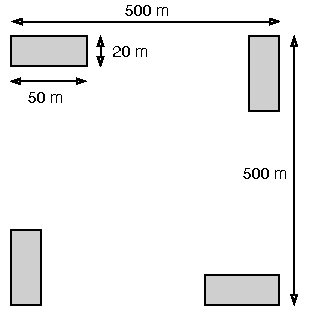
\includegraphics[width=0.5\textwidth]{schematic}
	\caption{Schematic diagram of plot layout within a site. Each 20$\times$50 m (0.1 ha) plot is shaded grey. Note that the plot dimensions are not to scale.}
	\label{schematic}
\end{figure}

Within each plot, the species and basal area of all trees with at least one stem $\geq$\stemSize{} cm DBH were recorded. Plot data were aggregated to the site level for analyses to avoid pseudo-replication. Each site covers an area of 500 m\textsuperscript{2}, matching that of the land surface phenology data used. We excluded sites where plots differed appreciably in vegetation composition, to ensure that all sites used in statistical analysis were representative of the vegetation within the 500 m\textsuperscript{2} area of vegetation. Using the Bray-Curtis dissimilarity index on species basal area data \citep{Faith1987}, we calculated the mean pairwise compositional distance between plots within each site. Sites were discarded when the mean pairwise compositional distance among plots within the site was greater than the mean pairwise compositional distance of all plots across all sites. This excluded \plotDistN{} sites.

\subsection{Vegetation composition and diversity} 

To classify variation in tree species composition we used agglomerative hierarchical clustering on species basal area data \citep{Kreft2010, Fayolle2014}. We excluded species with fewer than five records across all sites from this analysis, as very rare species can hinder meaningful cluster delineation. We used Ward's algorithm to define clusters \citep{Murtagh2014}, based on the Bray-Curtis distance between pairs of sites. We determined the optimal number of clusters by maximising the mean silhouette width among clusters \citep{Rousseeuw1987}. We described the vegetation types represented by each cluster using Dufr\^{e}ne-Legendre indicator species analysis \citep{Dufrene1997}. \Numberstringnum{\nCluster} vegetation types were identified during hierarchical clustering. The silhouette value of the clustering algorithm reached \silBest{}. 

While all vegetation types were present across Zambia, there was some spatial and climatic stratification (\autoref{site_map}). Three miombo woodland types were identified, each with different sets of secondary species, but all dominated by Detarioid species such as \textit{Brachystegia} spp. and \textit{Julbernardia} spp. (\autoref{clust_summ}). Uapaca miombo is largely absent from the southwest of the country, occurring predominantly in higher rainfall regions to the north and east. Cryptosepalum-dominated miombo is found more in the southwest of the country, possibly representing the drier ``Angolan miombo woodlands'' described by \citet{White1983}. Julbernardia miombo is common in cooler areas and is more climatically restricted than the other miombo woodland types. Combretaceae woodlands match the description of small stature Zambesian woodlands, as described by \citet{Dinerstein2017} and \citet{Chidumayo2001}. These woodlands are not dominated by the same archetypal Detarioideae tree species as the other miombo woodland vegetation types. These combretaceae woodlands occur over a wide climatic range, and contain some of the warmest sites in our dataset in the southeast of the country. The miombo woodland vegetation types are dominated by \textit{Brachystegia} spp. and \textit{Julbernardia} spp., with different secondary species. Median species richness and the range of species richness values per site is similar across vegetation clusters (\autoref{clust_summ}). 

\begin{figure}[H]
\centering
	\includegraphics[width=\textwidth]{site_map}
	\caption{Distribution of study sites, within Zambia (left), and in climate space (right). Sites are shown as triangles, coloured according to vegetation type cluster. Zambia is shaded according to mean growing season length during the period \modisStart{} to \modisEnd{}, estimated from the MODIS MCD12Q2 land surface phenology product, at 500 m spatial resolution \citep{MCD12Q2}. Growing season length is masked by the MODIS MCD12Q1 land cover map from 2015 \citep{MCD12Q1}, removing all pixels occurring in wetlands, croplands, water bodies, and urban areas. Climate space is represented by Mean Annual Temperature (MAT) and Mean Annual Precipitation (MAP), extracted from the WorldClim dataset at 30 arc second resolution \citep{Fick2017}. The shaded area in the right panel shows the climate space of Zambia, showing the density of pixels for given values of MAT and MAP. The ellipses in the right panel show the 95\% confidence interval for modelled climate space of each vegetation type cluster.} 
	\label{site_map}
\end{figure}

\setlength{\tabcolsep}{2pt} % Default table column sep width 
\input{out/clust_summ.tex}
\setlength{\tabcolsep}{4pt} % Default table column sep width 

To describe species diversity in each site, we calculated the Shannon-Wiener index ($H'$) from species basal area rather than individual abundance, as a measure of species diversity effectively weighted by a species' contribution to canopy occupancy and thus by contribution to the land surface phenological signal. $H'$ was transformed to the first order numbers-equivalent ($^1\!D$) of $H'$, calculated as $e^{H'}$ \citep{Jost2007}. We use $^1\!D$ as the primary measure of species diversity in our statistical models, and is subsequently referred to as species diversity. To describe average tree size, we calculated the quadratic mean of stem diameters per site \citep{Curtis2000}. The quadratic mean of diameter is directly related to basal area, unlike the arithmetic mean of diameter. It is thus a more appropriate descriptor of average tree size, as it scales linearly with volume and biomass.

\subsection{Land surface phenology}

To quantify phenology at each site, we used the MODIS MCD12Q2 v6.1 land surface phenology product \citet{MCD12Q2}. MCD12Q2 provides annual metrics describing land surface phenology, with a spatial resolution of \textasciitilde{500 m}. The phenological metrics in MCD12Q2 are derived from the 2-band MODIS EVI time series, with nadir BRDF adjusted surface reflectances. There are a number of land surface phenology products derived from MODIS vegetation indices. We chose MCD12Q2 as it has been used effectively in other studies in African woodlands to measure growing season period \citep{}. Additionaly, a previous comparison of MODIS-derived land surface phenology products showed that MCD12Q2 out-performed other products in predicting the start of the growing season in relation to ground observations \citep{Peng2017}. 

All sites were determined to have a single annual growing season according to the MCD12Q2 ``NumCycles'' metric. We used the ``Greenup'' and ``Dormancy'' metrics to define the growing season as the period when the EVI time series exceeds 15\% of the EVI amplitude for a given growing season (\autoref{ts_illus}). We used the ``Senescence'' and ``Maturity'' metrics to define the end/start of the green-up/senescence periods and the period maximum foliage cover as the period when the EVI time series exceeds 90\% of the EVI amplitude for that growing season. We used all years from \modisStart{} to \modisEnd{} and calculated mean values of growing season length, start of growing season date, end of growing season date, and length of the green-up and senescence periods for each site in our study.

\subsection{Precipitation and temperature data}

Precipitation data for each site was taken from the GPM IMERG Final Precipitation L3 1 day V06 product, which has a pixel size of 0.1\textdegree (11.1 km at the equator) \citep{IMERG}. Daily total precipitation was separated into three periods: precipitation during the growing season, precipitation in the 30 day period before the onset of the growing season (pre-green-up precipitation), and precipitation in the 30 day period before the onset of senescence at the end of the growing season (pre-senescence precipitation). 

There is no clear consensus on best practice for defining the limits of the rainy season \citep{Guan2014}. Here we followed the example of \citet{Stern1981} and \citet{Adole2018a}, variations of which have been used in several studies of African savanna-woodland phenology \citep{Ryan2017, Tadross2005, Mupangwa2011, Segele2005}. We first defined ``hydrological years'' for each site, bounded by the calendar months experiencing the lowest precipitation in each calendar year \citep{Ferijal2022}. Where multiple months tied for lowest precipitation, the month was chosen which would produce the shortest hydrological year. Note that hydrological years may be longer or shorter than a calendar year. The onset of the rainy season for each hydrological year was then defined as the start of the first period of \onsetPeriodOne{} days with more than \onsetPrecipOne{} mm total rainfall, followed by \onsetPeriodTwo{} days with more than \onsetPrecipTwo{} mm total rainfall. The end of the rainy season was defined as the start of the first period where where fewer than \Numberstringnum{\rainyDaysEnd} days within a \periodEnd{} day period received more than \rainyDef{} mm rainfall. \citet{Guan2014} compares other methods of estimating rainy season onset and end dates, and finds little functional difference between the method chosen here and other common methods. To validate our chosen definition of rainy season we checked that all season start and end dates occurred within 5 days of the dates where 10\% and 95\% of yearly cumulative rainfall were exceeded, for each hydrological year \citep{Adole2018a}. 

We calculated the lag between the onset of the growing season and the onset of the rainy season as the difference between these two dates. Similarly we calculated the lag between the end of the growing season and the end of the rainy season. These two metrics are referred to as ``green-up lag'' and ``senescence lag'' hereafter. To aid interpretation of statistical models, we reversed the sign of the green-up lag measurements, so that larger values indicate earlier pre-rain green-up.

Mean diurnal temperature range (Diurnal $\delta{}$T) was calculated for each site as the mean of monthly temperature range from the WorldClim database, using the BioClim variables (BIO2), with a pixel size of 30 arc seconds (926 m at the equator) \citep{Fick2017}, averaged across all years of available data (1970-2000).

\begin{figure}[H]
\centering
	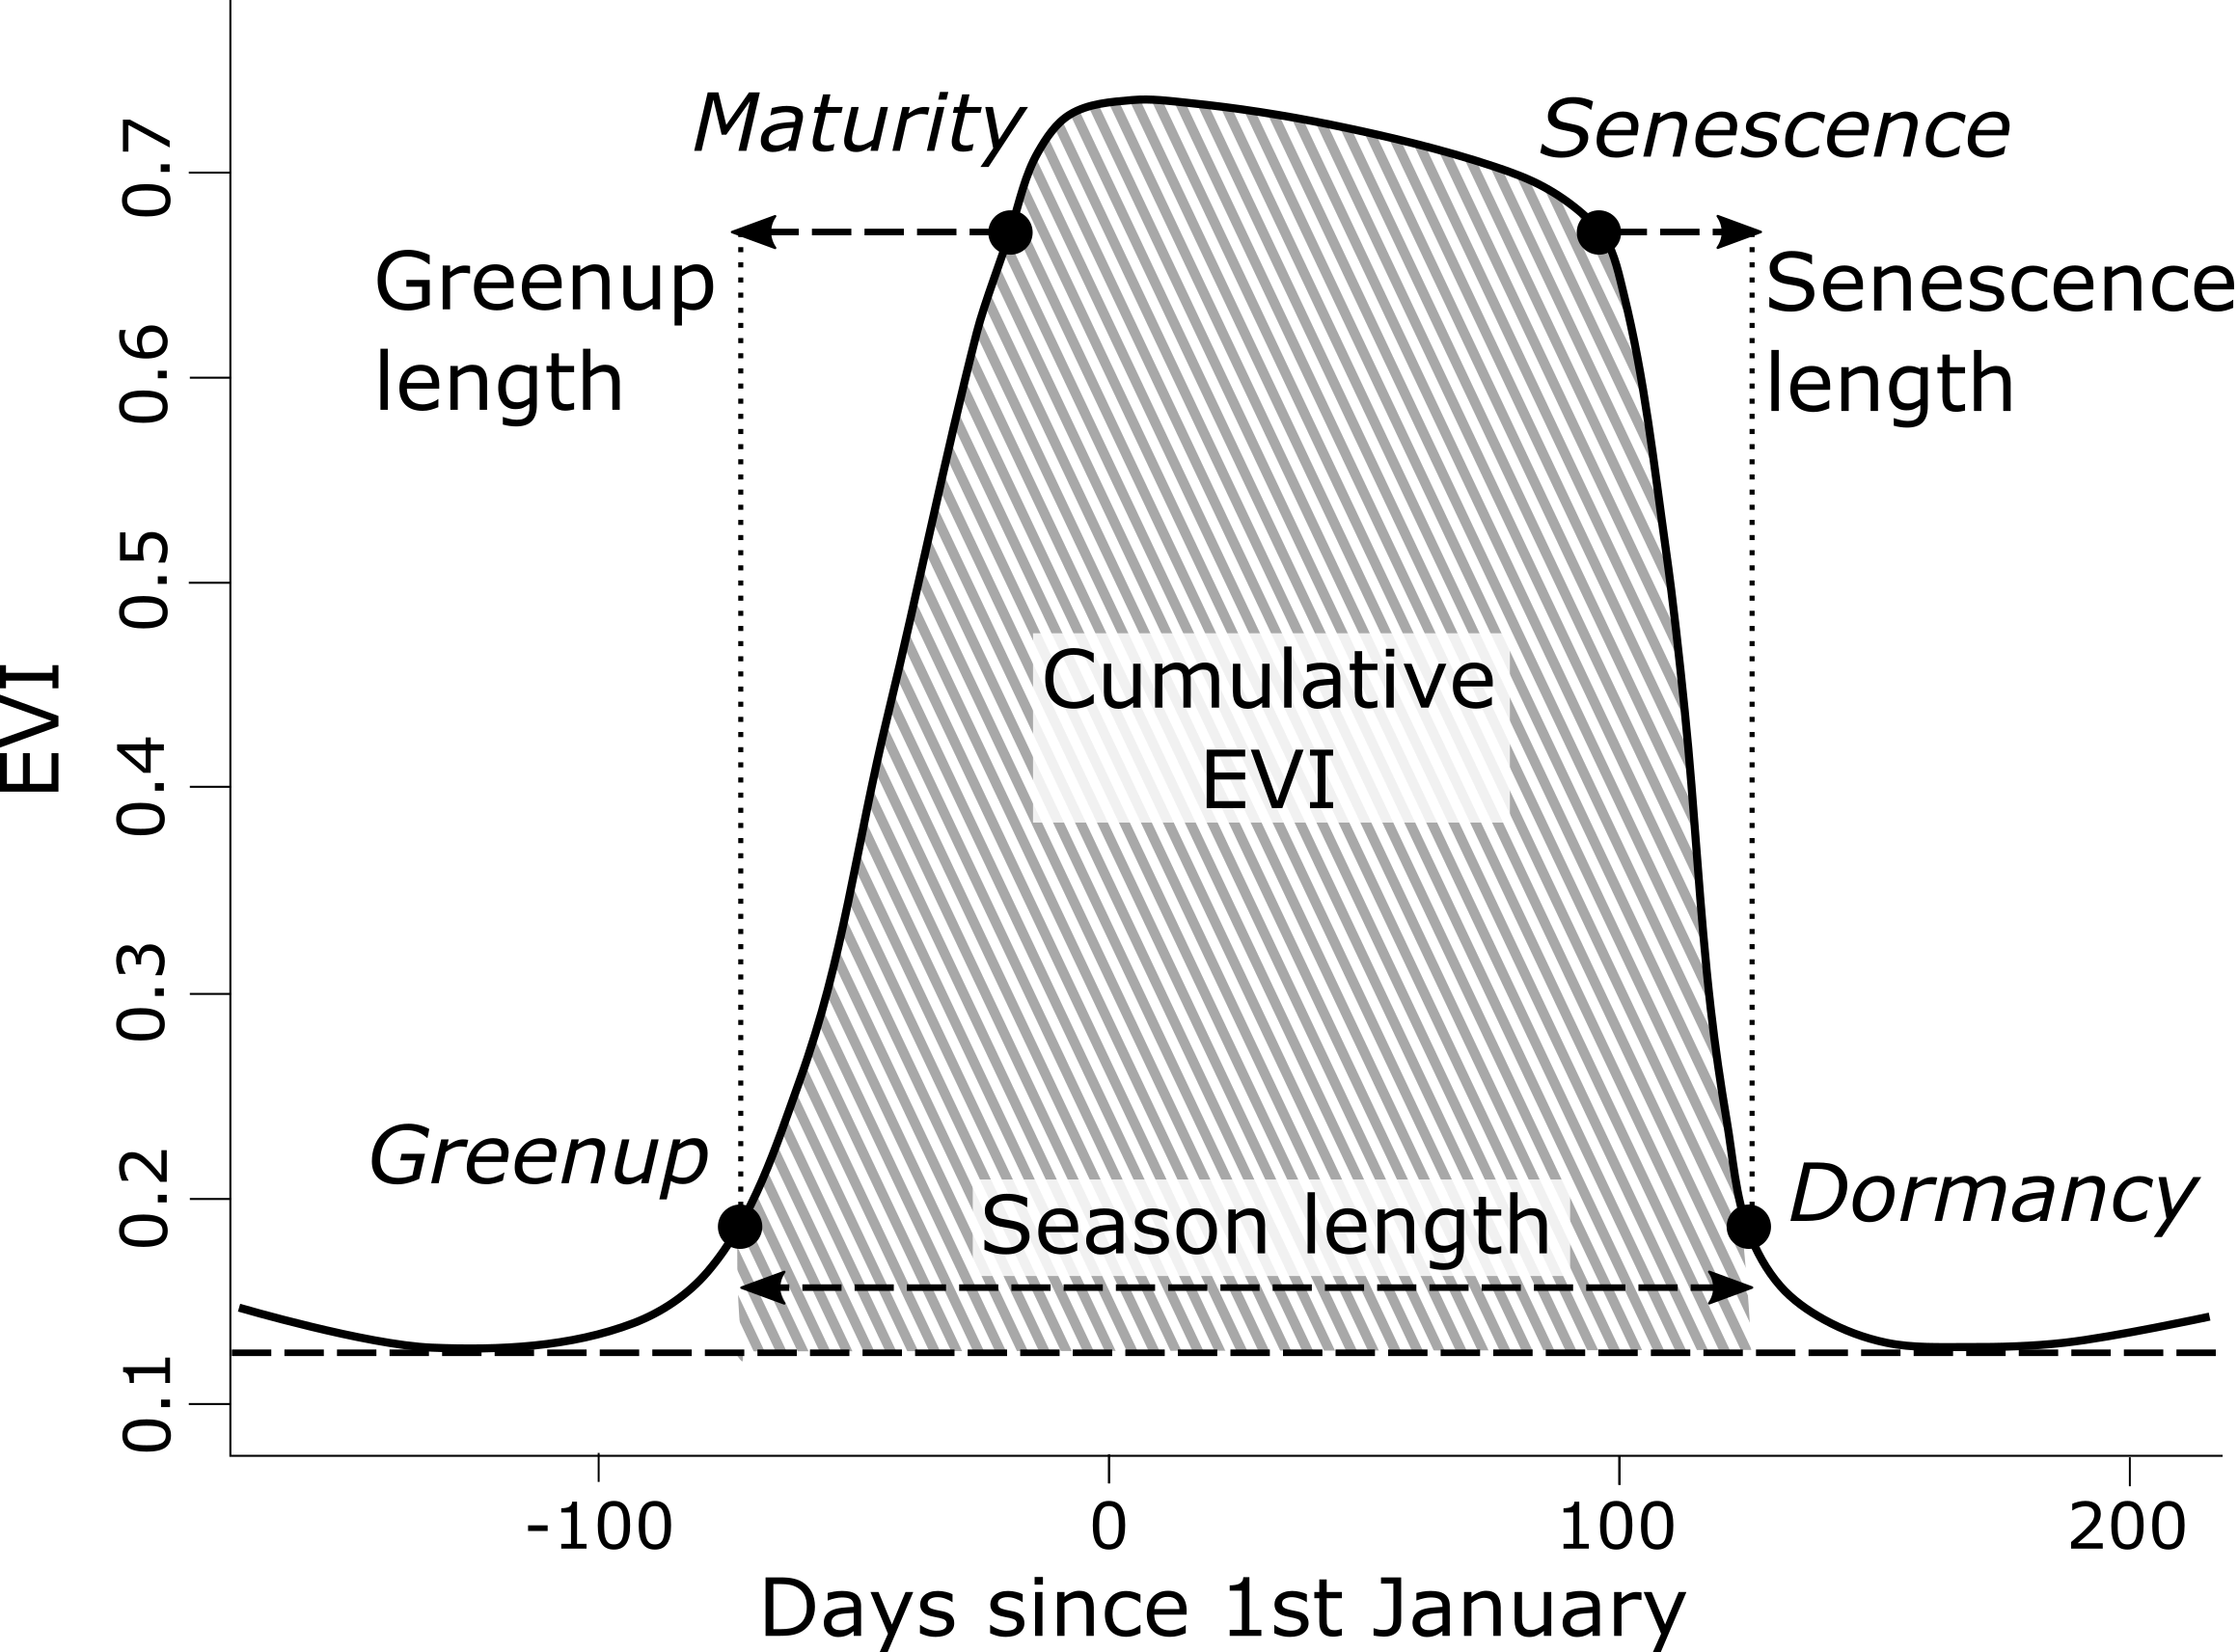
\includegraphics[width=0.8\textwidth]{ts_illus}
	\caption{Schematic diagram of hypothetical splined NBAR-EVI2 time series, from which metrics provided by the MCD12Q2 product are derived, illustrating the positions of phenological metrics used in this study. Cumulative EVI indicates the shaded area under the EVI curve for a given growing season, bounded by the ``Greenup'' and ``Dormancy'' dates. Adapted from \citep{Gray2022}.}
	\label{ts_illus}
\end{figure}

\subsubsection{Statistical modelling}

We used multivariate linear models to investigate the effect of tree species diversity, composition, and woodland structure on each phenological metric. We defined a maximal model structure including the explanatory variables of species diversity, quadratic mean of tree stem diameter, and relative abundance of Detarioid species, alongside climatic variables shown by previous studies to strongly influence patterns of foliage production and senescence: precipitation and diurnal temperature range. For models of growing season length and cumulative EVI we used total cumulative rainy season precipitation, for green-up lag and length of green-up period we used pre-green-up precipitation, and for senescence lag and length of senescence period we used pre-senescence precipitation. We included interaction terms for species diversity and mean stem diameter with vegetation type. We used the \texttt{dredge} function from the \texttt{MuMIn} R package to determine which combination of explanatory variables and their interactions best explained each phenological metric. \texttt{dredge} produces a suite of models containing all possible combinations of explanatory variables and their defined interactions. Candidate models were compared using the model log-likelihood, AIC (Akaike Information Criteria), and adjusted R\textsuperscript{2}. Where two similar models were within 2 AIC points of each other, the model with fewer terms was chosen as the best model, to maximise model parsimony. Explanatory variables in each model were standardised to Z-scores prior to modelling to allow comparison of slope coefficients within a given model.

We assessed standardised effect sizes for explanatory variables in each best model to determine the magnitude and direction of their effect on each phenological metric. To investigate variation in the role of species diversity and woodland structure on phenological metrics among vegetation types, we estimated marginal means for these explanatory variables for each of the vegetation types, if they appeared in the best model. We estimated marginal means using the \texttt{ggeffects} package in R. Estimating marginal means entails generating model predictions across values of a focal variable, while holding non-focal variables constant at their reference value.

To describe variation in land surface phenology among vegetation clusters we conducted a MANOVA using the phenological metrics as response variables, followed by post-hoc Tukey's tests between each pairwise combination of vegetation clusters per phenological metric, to test whether vegetation clusters differed significantly in their land surface phenology. All statistical analyses were conducted in R version 4.0.2 \citep{R2020}.

\section{Results}

Multi-variate linear models effectively predicted season length (R\textsuperscript{2} = \lengthRsq{}), green-up lag (R\textsuperscript{2} = \glagRsq{}) and senescence lag (R\textsuperscript{2} = \slagRsq{}), while green-up length (R\textsuperscript{2} = \grateRsq{}), senescence length (R\textsuperscript{2} = \srateRsq{}), and cumulative EVI (R\textsuperscript{2} = \cumviRsq{}) were poorly constrained even in the best models according to the model selection procedure. Tree species diversity exhibited strong positive effects on both season length (H\textsubscript{1}) and green-up lag (H\textsubscript{2}) (\autoref{mod_slopes}). Despite the best model for cumulative EVI including species diversity as an explanatory variable, the slope of this effect was insignificant, with a wide standard error.

Average tree size, measured by the quadratic mean of stem DBH per site, was not a significant predictor of any phenological metric (H\textsubscript{3}). While it was included in the best model for cumulative EVI, with a marginally positive effect, this effect was not significant. The relative basal area abundance of species from the Fabaceae family, subfamily Detarioideae, was a significant predictor of season length and green-up lag (H\textsubscript{4}).

The slope of some relationships between vegetation metrics and phenological metrics varied among vegetation types (\autoref{mod_marg}). The strong positive effect of species diversity on season length and green-up lag was shared among all vegetation types. Relative basal area abundance of Detarioideae species had a positive effect on season length across all vegetation types. The effect of Detarioideae relative basal area abundance on green-up lag was marginally negative in Uapaca miombo, but clearly positive in all other vegetation types. Variation in the effect of species diversity on senescence length also varied by vegetation type, with a negligible effect of this variable observed in Cryptosepalum miombo, but positive effects in other vegetation types.
 
A MANOVA including all phenological metrics showed a significant difference among vegetation clusters (\phenManova{}). Combretaceae woodlands had a significantly shorter growing season length than the other vegetation types, along with significantly shorter periods of green-up and senescence (\autoref{boxplots}). The majority of plots, regardless of vegetation type, exhibited some degree of pre-rain green-up. Across all sites, the mean lag between green-up and the onset of seasonal rains was \greenLagMean{}.

\begin{figure}[H]
\centering
	\includegraphics[width=\textwidth]{mod_slopes.pdf}
	\caption{Standardised slope coefficients for the best model of each phenological metric. Slope estimates are $\pm$1 standard error. Slope estimates where the interval does not overlap zero are considered to be significant effects and are marked by asterisks. Note that standardised slope coefficients should not be compared among models shown in the different panels.}
	\label{mod_slopes}
\end{figure}

\begin{figure}[H]
\centering
	\includegraphics[width=\textwidth]{mod_marg.pdf}
	\caption{Standardised marginal effects of tree species diversity on each of the phenological metrics, using the maximal mixed effects model, for each vegetation cluster. Dotted lines represent 95\% confidence intervals. Units of `d' are number of days.}
	\label{mod_marg}
\end{figure}

\begin{figure}[H]
\centering
	\includegraphics[width=\textwidth]{boxplots.pdf}
	\caption{Boxplots of the six phenological metrics used in the study, grouped by vegetation type. Letters not shared among vegetation types denote that these vegetations types were identified as significantly different by post-hoc Tukey's HSD tests derived from the MANOVA of phenological metrics by cluster. Units of `d' are number of days.}
	\label{boxplots}
\end{figure}

\section{Discussion}

% GOOD
In this study we have demonstrated clear and measurable effects of tree species diversity, composition and structure on various metrics of land surface phenology in deciduous woodlands across Zambia. We have shown that tree species diversity led to an increase in growing season length across wooodland compositional types. Additionally, species diversity caused the onset of greening to occur earlier with respect to the start of the rainy season. Our study lends support for a general positive effect of tree species diversity on primary productivity in southern African deciduous woodlands, with species rich woodlands exhibiting a longer growing season.

% GOOD
Our finding that species diversity caused earlier pre-rain green-up suggests that diverse woodlands are more resilient to temporal variations in the onset of seasonal rainfall. This provides early forage for herbivores \citep{Morellato2016}, and provides facilitative effects such as cover and hydraulic lift which benefit understorey plants \citep{Domec2010, Yu2015}. Our results highlight the role of tree species diversity as a driver of key ecosystem processes, which affect ecosystem structure, the wildlife provisioning role, and gross primary productivity. 

% GOOD
The basal area abundance of trees from the Fabaceae family, subfamily Detarioideae, had a positive effect on season length and green-up lag. Previous studies have noted the importance of Detarioideae species in driving woody productivity in miombo woodlands \citep{Ryan2017}, where they dominate the woodland canopy \citep{Godlee2021, Chidumayo2001}. This study supports those previous observations. Given their tendency to create deep root networks \citep{Zhou2020}, and their conservative leaf economic spectrum traits \citep{Wigley2016}, we suggest that compared to other taxonomic groups, Detarioideae species are able to access deep groundwater reserves to green-up before seasonal rainfall begins.

% GOOD
The lag between the end of the growing season and the end of the rainy season was not strongly influenced by tree species diversity. \citet{Cho2017} found that tree cover, measured by MODIS LAI data, had a significant negative effect on senescence rates in woodlands in South Africa, which have similar climatic conditions to the sites in our study. In most woodlands, including sparse savannas, while the onset of the growing season is often driven by tree photosynthetic activity, which may precede the onset of precipitation, the end of the growing season is conversely driven by the understorey grass layer \citep{Cho2017, Guan2014}. Grass activity is more reactive to short-term changes in soil moisture than tree activity, and may oscillate within the senescence period \citep{Archibald2007}. This may explain the lack of a strong precipitation signal for senescence lag and length of the senescence period in our models.

% WHy didn't we find strong models for length of of greening and senescence periods?

% Good para, no changes
Other studies both globally and within southern African woodlands have largely ignored patterns of senescence, instead focussing patterns of green-up \citep{Gallinat2015}. Most commonly, these studies simply correlate the decline of rainfall with senescence \citep{Stevens2016, Guan2014}, but our best model suggests that diurnal temperature range is a stronger determinant of the end of the growing season than precipitation. Diurnal temperature range effectively measures mean daily temperature variability. We suggest that diurnal temperature fluctuations, particularly minimum night time temperatures, may provide cues for senescence toward the end of the rainy season. In temperate ecosystems which experience autumn senescence, lower night time temperatures have been shown to increase the rate of senescence and thus decrease senescence period length \citep{Michelson2017, Escamilla2020}, thus leaves remain green for longer when the diurnal temperature range is smaller. Similarly, our models showed that larger diurnal temperature range caused earlier pre-rain green-up, and possibly acts as a cue to initiate the growing season as well.

% Good para, no changes
Alternatively, \citet{Zani2020} suggests that in resource limited environments, senescence times may largely be set by the preceding photosynthetic activity and sink-limitations on growth. For example, limited nutrient supply may prohibit photosynthesis late in the season if the preceding photosynthetic activity has depleted that supply. \citet{Reich1992} suggested that there are many direct constraints on leaf life-span such as drought and herbivory, especially in the seasonally dry tropics, which would lead to timing of senescence being set largely by the time of bud-burst. Our study corroborates this theory, showing that precipitation across the entire rainy season was a better predictor of senescence lag than pre-senescence precipitation. We also found a moderate positive correlation between green-up lag and senescence lag across all vegetation types, indicating that later green-up allows later senescence (\autoref{phen_bivar}).

% Good para, no changes
Our finding that species diversity strongly affects patterns of land surface phenology in seasonally dry tropical woodlands provides earth surface system modellers with a means to better understand how future changes in species diversity and composition will affect land surface phenology. Incorporating predictions of biotic change into earth system models has been limited \citep{Ahlstrom2015, Bodegom2011} until now for two main reasons. Firstly, there are large uncertainties in the effects of diversity on ecosystem function, e.g. gross primary productivity (GPP). Secondly, until recently there has been a major paucity of ground data on community composition \citep{}. Our study comes at a pertinent time when plot-based vegetation monitoring networks have become sufficiently widespread \citep{}, and remotely sensed proxies of tree species diversity are becoming sophisticated enough \citep{} to be of real use to earth system modellers. Our study provides a link by demonstrating a strong relationship between species diversity and phenological metrics, particularly growing season length which is itself closely correlated with GPP \citep{Sjostrom2011}. 

\section{Conclusion}

We explored how tree species diversity, composition and structure of deciduous woodlands influence land surface phenology across Zambia. We showed that species diversity clearly drives longer growing seasons and promotes earlier pre-rain green-up, across all woodland compositional types studied here. The abundance of species from the Fabaceae family, subfamily Detarioideae had a consistent positive effect on season length and caused earlier pre-rain green-up, supporting suggestions of their role in driving pre-rain green-up in southern African miombo woodlands. Contrary to our expectations, we did not find evidence for an effect of mean tree size on land surface phenology, indicating that phenological adaptation of species is not merely correlated with maximum tree size. Finally, we have demonstrated variation in phenological patterns among woodland compositional types within Zambia that are commonly not distinguished in earth system models. 

Our results lend further support to an already well established corpus of study on the positive effect of species diversity on ecosystem function. Additionally, our results provide evidence for earth-system modellers, demonstrating the importance of community composition and diversity in determining patterns of land surface phenology. As reliable data on plant community composition becomes available across larger spatial scales and at higher spatial resolution, we hope that these data can be included in models of land-atmosphere mass and energy exchange to improve their predictive power.

\printbibliography

\section{Supplementary Material}
\beginsupplement

\begin{figure}[H]
\centering
	\includegraphics[width=\textwidth]{phen_bivar}
	\caption{Scatter plots showing pairwise comparisons of the six phenological metrics used in this study, extracted from the MODIS MOD13Q1 product \citep{MOD13Q1}. Points represent study sites and are coloured by vegetation cluster. Linear regression line of best fit for all sites is shown as a black line, while linear regressions are shown for each vegetation cluster as coloured lines. The units of `d' are the number of days.}
	\label{phen_bivar}
\end{figure}

\end{document}

